

\begin{figure}
\centering
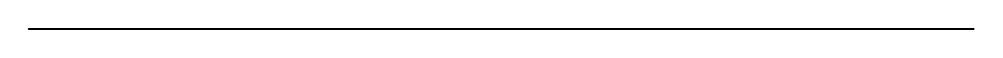
\begin{tikzpicture}[scale=1,cap=round]
\tkzInit[xmin=-4, xmax=4, ymin=0, ymax=3]
\tkzClip
%Draw circle
\tkzDefPoint(0,0){O} %define origin
\tkzDefPoint(-2,0){x1}
\tkzDefPoint(2,0){x2}
\tkzDefPoint(-3,0){y1}
\tkzDefPoint(3,0){y2}
\tkzDefPoint(-2.25,0){c1}
\tkzDefPoint(2.25,0){c2}

\tkzDrawCircle[thick, fill=gray!30](O,y1){circleOy}
\tkzDrawCircle[thick, fill=white](O,x1){circleOx}

\tkzDrawCircle[thick, fill=white](x1,c1){circlex1}
\tkzDrawCircle[thick, fill=white](x2,c2){circlex2}
\tkzDrawCircle[thick, fill=white](y1,c1){circley1}
\tkzDrawCircle[thick, fill=white](y2,c2){circley2}

\draw[thick] (-6, 0) -- (6, 0); %horizontal line

\end{tikzpicture}
\caption{A fundamental domaine of a punctured torus}
\end{figure}
